\section{Architektura hlubokého modelu variačního autoenkodéru}
Model variačního autoenkodéru je pro účely tohoto experimentu navrhnutý tak, aby byl schopen flexibilně řešit různé úlohy generativního modelování obrazových dat.
V rámci této kapitoly je popsána konstrukce, trénování a analýza modelu variačního autoenkodéru pro \textbf{ilustrační řešení} úlohy generativního modelování obrazových dat MNIST.

Byla vytvořena třída modelu variačního autoenkodéru v jazyce Python, která jako parametry přijímá konfiguraci konvolučních vrstev enkodér a dekodér modulů, spolu s očekávaným tvarem trénovacích dat.
Tato stejná třída modelu variačního autoenkodéru by tak šla využít i pro generativní úlohu obrazových dat na zcela jiném datasetu.

Kompletní zdrojové kódy modelu a vizualizací nabízí \autoref{app:vae_model_source_code}.

Tato sekce je zaměřena na návrh a principy fungování jednotlivých modulů tohoto modelu, konkrétně:
\footnote{Model variačního autoenkodéru se od prostého autoenkodéru (viz \autoref{chap:autoencoder}) liší zejména v \textbf{enkodér modulu} a \textbf{ztrátové funkci} (viz \autoref{sec:vae_objective}).} jsou nutné následující moduly, resp. vrstvy:
\begin{itemize}
    \item Model enkodér modulu
    \item Model dekodér modulu
    \item Reparametrizační vrstva
    \item Ztrátová funkce
\end{itemize}

V této sekci jsou tyto moduly propojeny s teoretickými aspekty variačního autoenkodéru z předchozích kapitol a postupně implementovány za účelem řešení úlohy generativního modelování obrazových dat na datové sadě MNIST.
\autoref{sec:vae_prepared_model} pak prezentuje výsledný model variačního autoenkodéru, který je připraven pro trénování.

Sekce se naopak, vzhledem k omezením stanoveným rozsahem práce, \textbf{nezabývá} popisem nástrojů použitých pro vytvoření popisované třídy modelu variačního autoenkodéru, které jsou pro účely práce považovány za doprovodné.

\subsection{Enkodér}
\label{sec:vae_model_encoder}
U prostého autoenkodéru je každý vstup mapován přímo na \textbf{pouze jeden bod} v latentním prostoru (tedy výsledný latentní prostor není spojitý).
Naopak ve variačním autoenkodéru je každý vstup mapován na (vícerozměrné) normální rozdělení okolo konkrétního bodu v latentním prostoru, jak ukazuje \autoref{fig:vae_encoder_difference}.

\begin{figure}[H]
    \centering
    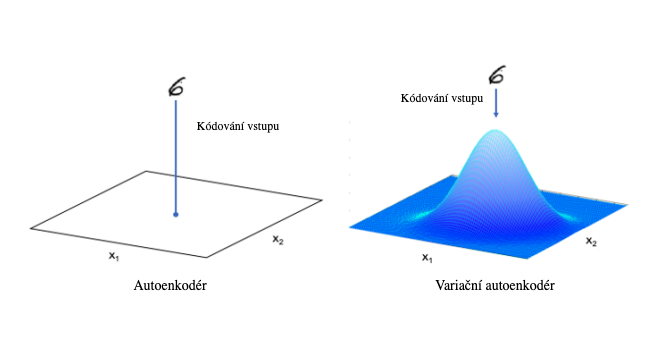
\includegraphics[width=\textwidth]{figures/vae_encoder_module.png}
    \caption{Rozdíl mezi enkodér modulem autoenkodéru a enkodér modulem variačního autoenkodéru. Umožňuje vzorkování ze spojitého latentního prostoru VAE. Obrázek převzat z \textcite{Foster2023}.}
    \label{fig:vae_encoder_difference}
\end{figure}

Pro připomenutí, jak plyne z \autoref{sec:vae_encoder}, enkodér modul variačního autoenkodéru \textbf{zakóduje každý vstup do dvou vektorů} – \lstinline{z_mean} a \lstinline{z_log_var}
\footnote{Jak víme z \autoref{sec:vae_optimization} enkodér modul předpokládá že \textbf{neexistuje korelace mezi žádnou z dimenzí latentního prostoru} a tím pádem je výsledná kovarianční matice diagonální. V důsledku tak enkodér modulu stačí mapovat každý vstup na vektor středních hodnot a vektor rozptylu.},
ze kterých je následně v latentním prostoru \textbf{sestaveno} (vícerozměrné) \textbf{normální rozdělení}, kde:
\lstinline{z_mean}: střední hodnota rozdělení a \lstinline{z_log_var}: logaritmus rozptylu (každé z dimenzí).

Pro vytvoření kódu vstupního obrázku do konkrétní latentní proměnné $z$ v latentním prostoru modelu lze z takto vzniklé distribuce vzorkovat pomocí reparametrizační vrstvy modelu. Tento proces detailněji popisuje \autoref{sec:vae_model_reparametrization_layer}.

Model enkodér modulu variačního autoenkodéru je pro účely tohoto experimentu definován následující konfigurací vrstev \footnote{Počet vrstev vychází z \textcite{Kingma2014} a jejich konfigurace byla následně modifikována a rozšířena na základě minimalizace ztrátové funkce a prevence přeučení. Detailnější popis nabízí \autoref{sec:vae_model_loss_function}.}:
\begin{enumerate}
    \item \textbf{Vstupní vrstva}\footnote{\lstinline{input_dim} odpovídá jedné číslici MNIST.}: \mint{python}|Input(shape=(28, 28, 1), name='encoder_input')|
    \item \textbf{Konvoluční vrstva}: \mint{python}|Conv2D(filters=32, kernel_size=3, strides=1, padding='same')|
    \item \textbf{Konvoluční vrstva}: \mint{python}|Conv2D(filters=64, kernel_size=3, strides=2, padding='same')|
    \item \textbf{Konvoluční vrstva}: \mint{python}|Conv2D(filters=64, kernel_size=3, strides=2, padding='same')|
    \item \textbf{Konvoluční vrstva}: \mint{python}|Conv2D(filters=64, kernel_size=3, strides=1, padding='same')|
    \item \textbf{Vyhlazovací vrstva}: \mint{python}|Flatten()(x)|
\end{enumerate}

Schematické zobrazení vrstev enkodér modulu ilustruje \autoref{fig:vae_model_encoder}.
\begin{figure}[H]
    \centering
    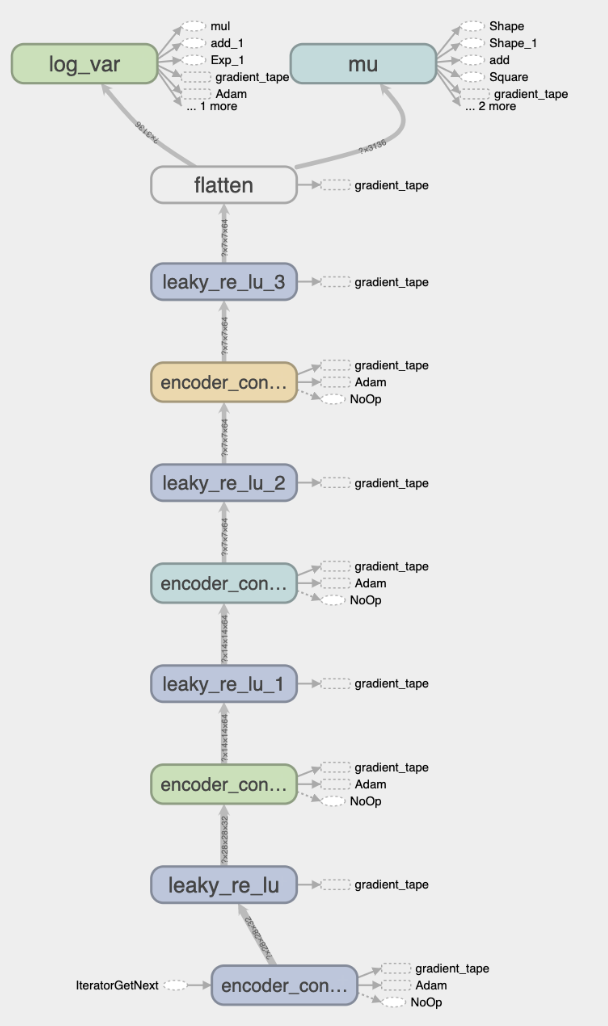
\includegraphics[height=0.63\textheight]{figures/vae_model_encoder.png}
    \caption{Diagram enkodér modulu VAE pro generování MNIST číslic.}
    \label{fig:vae_model_encoder}
\end{figure}

\subsection{Dekodér}
\label{sec:vae_model_decoder}
Dekodér modul variačního autoenkodéru je principem identický k dekodéru prostého autoenkodéru.
Model denkodér modulu variačního autoenkodéru je pro účely tohoto experimentu definován následující konfigurací vrstev\footnote{Počet vrstev vychází z \textcite{Kingma2014} a jejich konfigurace byla následně modifikována a rozšířena na základě minimalizace ztrátové funkce a prevence přeučení. Detailnější popis nabízí \autoref{sec:vae_model_loss_function}.}:

\begin{enumerate}
    \item \textbf{Vstupní vrstva}:\footnote{\emph{shape} odpovídá dimenzi latentního prostoru (pro obrázky MNIST číslic 2D).} \mint{python}|Input(shape=2, name='encoder_input')|
    \item \textbf{Dekonvoluční vrstva}: \mint{python}|Conv2DTranspose(filters=64, kernel_size=3, strides=1, padding='same')|
    \item \textbf{Dekonvoluční vrstva}: \mint{python}|Conv2DTranspose(filters=64, kernel_size=3, strides=2, padding='same')|
    \item \textbf{Dekonvoluční vrstva}: \mint{python}|Conv2DTranspose(filters=32, kernel_size=3, strides=2, padding='same')|
    \item \textbf{Dekonvoluční vrstva}: \mint{python}|Conv2DTranspose(filters=1, kernel_size=3, strides=1, padding='same')|
    \item \textbf{Vyhlazovací vrstva}: \mint{python}|Flatten()(x)|
\end{enumerate}

\textbf{Vstupem pro dekodér modul je výstup enkodér modulu} VAE – tedy logaritmus rozptylu (\emph{\lstinline{z_log_var}}) a střední hodnota (\emph{\lstinline{z_mean}}), ze kterých je následně sestavena distribuce pro generování zcela nových výstupů.

\subsection{Reparametrizační vrstva}
\label{sec:vae_model_reparametrization_layer}
Reperametrizační vrstva modelu variačního autoenkodéru implementuje reparametrizační trik dle \autoref{sec:reparametrization_trick}.
Přičemž pro připomenutí, $\epsilon$ je bod náhodně vzorkovaný z normovaného normálního rozdělení.
Právě $\epsilon$ hraje při trénování variačního autoenkodéru důležitou roli, jelikož transformuje vzorkovací proces na diferenciovatelnou operaci (a této vlastnosti je využito při následné optimalizaci modelu, viz \autoref{sec:vae_model_loss_function}).


U variačního autoenkodéru je vzorkován náhodný bod z $\epsilon$-okolí \lstinline{z_mean}.
Tedy dekodér musí při trénování zajistit, aby všechny body v tomto okolí produkovaly výstup (obrázek) který je \emph{velmi podobný} vstupu, nebo má alespoň podobný sémantický význam.
Popsanou operaci v reparametrizační vrstvě modelu zachycuje \autoref{code:vae_reparametrization_layer}.

\begin{figure}[H]
    \inputminted[linenos]{python}{code_snippets/vae_reparametrization.py}
    \caption{Reparametrizační vrstva modelu variačního autoenkodéru.}
    \label{code:vae_reparametrization_layer}
\end{figure}

Toto je velmi elegantní vlastnost variačního autoenkodéru, která zajistí že i v případě, kdy je při vzorkování zvolen bod, který dekodér modul variačního autoenkodéru doposud nikdy \emph{neviděl}, s vysokou pravděpodobnostní bude výstupem dobře formovaný obrázek.
Tedy \textbf{variačnímu autoenkodéru je umožněno generovat data, která nebyly součástí trénovací množiny, ale nesou stejné charakteristiky jako vstupní data}.
Syntéza takovýchto dat je jedna z hlavních účelů oblastí generativního modelovaní.
Tuto vlastnost detailněji zkoumá \autoref{sec:vae_model_latent_space_observation}, která se věnuje pozorování latentního prostoru naučeného modelu.

\subsection{Ztrátová funkce}
\label{sec:vae_model_loss_function}
Ztrátová funkce modelu variačního autoenkodéru implementuje postup dle \autoref{eq:vae_elbo}.
Model VAE tedy \textbf{minimalizuje součet hodnoty chyby rekonstrukce a hodnoty KL divergence}.

Pro rekapitulaci \autoref{sec:kl_divergence}, KL divergence vyjadřuje míru \textbf{nepodobnosti} (resp. \emph{"vzdálenosti"}) mezi pravděpodobnostními distribucemi.
U variačního autoenkodéru chceme měřit jak moc se liší normální rozdělení s parametry \lstinline{z_mean} a \lstinline{z_log_var} oproti normovanému normálnímu rozdělení.
Prvek KL divergence tedy penalizuje umělou neuronovou síť modelu za takové kódování vstupních dat (jehož výsledkem je \lstinline{z_mean} a \lstinline{z_log_var}), které se \textbf{výrazně liší} od parametrů normované normálního rozdělení.
Tento prvek KL divergence tak hraje při trénování modelu důležitou roli, jelikož \emph{nutí} všechny distribuce s parametry, které jsou výsledkem kódování, \emph{podobat se} normovanému normálnímu rozdělení. 
V důsledku existuje \textbf{menší šance} že zformovaný \textbf{latentní prostor model bude obsahovat} \emph{značné} \textbf{mezery} mezi klastry latentních proměnných (jak ukazuje \autoref{sec:vae_model_latent_space_observation}).
Ve snaze o minimalizaci ztrátové funkce modelu se totiž enkoder modul pokouší o efektivní a symetrické využití prostoru v okolí počátku latentního prostoru.

Ztrátová funkce rovněž musí hledat \textbf{rovnováhu mezi hodnotou chyby rekonstrukce a hodnotou KL divergence}.
Udělení příliš velké váhy jednomu z těchto prvků by mělo za důsledek ztrátu kýženého regulačního efektu latentního prostoru a vzniklý model variačního autoenkodéru by nabýval stejných problémů, jako prostý autoenkodér.
Zajištění konvergence obou prvků je tak důležitou součástí trénovacího procesu modelu variačního autoenkodéru a vede k chtěné vlastnosti spojitého latentního prostoru, která umožňuje variačnímu autoenkodéru generovat i takové vzorky dat, které nebyly součástí trénovací množiny.

Logika trénovacího kroku modelu variačního autoenkodéru zahrnuje dopředný průchod, výpočet hodnoty ztrátové funkce a aktualizaci metrik modelu.
Trénovací krok modelu definuje \autoref{code:vae_loss_function}.

\newpage
\begin{figure}[H]
    \inputminted[linenos]{python}{code_snippets/vae_loss_function.py}
    \caption{Trénovací krok modelu variačního autoenkodéru.}
    \label{code:vae_loss_function}
\end{figure}


Kde:
\begin{itemize}
    \item \emph{Řádek č. 3}: Volá enkodér modul VAE za účelem získání kódu vstupních dat (tedy parametrů pravděpodobnostní distribuce).
    \item \emph{Řádek č. 4}: Realizuje \textbf{reparametrizační trik} dle \autoref{sec:reparametrization_trick} za účelem získání vzorku z latentního prostoru na základě parametrů jeho rozdělení pravděpodobnosti.
    \item \emph{Řádek č. 5}: Generuje rekonstrukci vstupních dat (v tomto případě obrázku MNIST číslice) na základě získaných latentních proměnných voláním dekodér modulu VAE.
    \item \emph{Řádek č. 7 - 9}: Realizuje gradientní optimalizaci dle \autoref{eq:vae_final_objective} výpočtem chyby rekonstrukce vygenerovaného vzorku vůči vstupním datům.
    \item \emph{Řádek č. 10}: Spočte KL divergenci mezi pravděpodobnostní distribucí latentních proměnných (s parametry \lstinline{z_mean}, \lstinline{z_log_var} ) a normovaným normálním rozdělením.
    \item \emph{Řádek č. 11}: Udává celkovou hodnotu ztrátové funkce dle \autoref{eq:vae_elbo}, respektive součet hodnoty chyby rekonstrukce a hodnoty KL divergence.
    \item \emph{Řádek č. 13}: Spočte gradienty vah neuronů dle \autoref{eq:vae_final_objective} s ohledem na celkovou hodnotu ztrátové funkce.
    \item \emph{Řádek č. 14}: Realizuje stochastická gradientní optimalizaci (s ohledem na již spočtené gradienty) dle \autoref{alg:reparam_trick}.
    \item \emph{Řádek č. 16 - 24}: Při každém trénovacím kroku aktualizuje a propaguje metriky ztrátové funkce na instanci VAE modelu.
\end{itemize}

\subsection{Výsledný model}
\label{sec:vae_prepared_model}
\autoref{code:vae_mnist_model} zachycuje konfiguraci instance VAE modelu pro úlohu generativního modelování obrazových dat MNIST.
Při instanciaci jsou jako parametry modelu předány konfigurace konvolučních vrstev enkodéru, resp. dekodéru přesně dle \autoref{sec:vae_model_encoder}, resp. \autoref{sec:vae_model_decoder}.

\begin{figure}[H]
    \inputminted[linenos]{python}{code_snippets/vae_model.py}
    \caption{Instanciace navrhnutého modelu VAE pro úlohu generativního modelování obrazových dat MNIST.}
    \label{code:vae_mnist_model}
\end{figure}

Kde:
\begin{itemize}
    \item \emph{Řádek 4}: Definuje rozměry (\emph{dimensions}) vstupních dat, kterou má VAE očekávat. V tomto případě pro MNIST číslice $28 \times 28$ px a 1 barevný kanál.
    \item \emph{Řádek 5}: Definuje požadovanou dimenzi latentního prostoru.
    \item \emph{Řádek 6 - 8}: Udává konfiguraci konvolučních vrstev modelu enkodér modulu dle \autoref{sec:vae_model_encoder}.
    \item \emph{Řádek 9 - 11}: Udává konfiguraci konvolučních vrstev modelu dekodér modulu dle \autoref{sec:vae_model_decoder}. 
\end{itemize}

